\documentclass[UTF8]{ctexart}

\usepackage{listings,xcolor}
\usepackage{graphicx}
\usepackage[a4paper,left=25.4mm,right=25.4mm,top=29.8mm,bottom=29.8mm]{geometry}

\lstset{numbers=left,
    commentstyle=\color{blue!50},
    columns=flexible}

\title{作业三:Avl树 —— 输出给定区间内的所有元素}

\author{张竣凯 \\ 3210300361 \\ 数学与应用数学}

\begin{document}

\maketitle

Write a function that takes as input a binary search tree, T, and two keys, k1 and k2,
which are ordered so that k1 ≤ k2, and prints all elements X in the tree such that
k1 ≤ Key(X) ≤ k2. Do not assume any information about the type of keys except
that they can be ordered (consistently). Your program should run in O(K + logN)
average time, where K is the number of keys printed. Bound the running time of
your algorithm.

\begin{flushright}
——摘自课本习题4.37
\end{flushright}

\section{设计思路}

\subsection{在 AVLTree.h 添加 printbetween 函数}

\begin{lstlisting}[language={[ANSI]C++}]
void printbetween( AvlNode *t , const Comparable & k1, const Comparable & k2)
{
    if( t == nullptr || t -> element < k1)
        return;
        
    else if( t -> element > k2 )
        printbetween( t -> left, k1, k2 );
    
    else
        printbetween( t -> left, k1, k2 );
        cout << t -> element << " ";
        printbetween( t -> right, k1, k2 );
}
\end{lstlisting}

\hphantom 空用于将给定区间内的所有元素打印出来,参数分别为AvlNode *t、Comparable \& k1以及Comparable \& k2,初始的t指向根节点。\\

\hphantom 空若t为空指针或t指向的元素小于k1,则什么都不做就直接返回;\\

\hphantom 空若t指向的元素大于k2,则进行函数迭代,此时代入函数的新t为旧t的左节点;\\

\hphantom 空若遇到除了以上提到的几种情况,则先进行函数迭代,此时代入函数的新t为旧t的左节点,接着打印出旧t指向的元素,最后再进行函数迭代,此时代入函数的新t为旧t的右节点。

\subsection{在 main.cpp 中编写 test 函数}

\begin{lstlisting}[language={[ANSI]C++}]
void test(int N) 
{
    clock_t start, finish;
    int k1, k2;
    AvlTree<int> T;
    for( int i = 1; i <= N; i++)
        T.insert(i);
    k1=1;
    k2=N/10;
    for( ; k2 <= N; k2 += N/10)
        cout << "当 k1 = " << k1 << ",k2 = " << k2 << " 时:" << endl;
        cout << "区间内的数据:";
        start = clock();
        T.printbetween( k1, k2 );
        finish = clock();
        cout << endl;
        cout << "打印出区间内数据的所需时间为: "<< double(finish - start)*1000 / 
                              CLOCKS_PER_SEC << "毫秒。" << endl;
        cout << endl;
    return;
}
\end{lstlisting}

\hphantom 空测试用的代码大同小异,故编写test函数以减少代码复制,参数为题目中的N。\\

\hphantom 空该函数应用了ctime库记录函数实际运行所需的时间,同时也使用了random库来随机选取小于N的两个数k1与k2,且k1$≤$k2。函数内部创建了一个AvlTree T,储存元素类型为整型int,并且通过for循环将1至N依次insert到T里,完成打印给定区间内的所有元素后,输出函数实际运行所需的时间。

\subsection{在 main.cpp 中编写 main 函数}
\hphantom 空调用事先写好的test函数,且可控制N的大小

\subsection{尽可能地使用引用\&以及充分考虑必要的const限制}
\hphantom 空以便于减少内部复制和提高安全性

\section{理论分析}

AVL树又称为高度平衡树,对于有N个节点的AVL树,其深度为$logN$,于是在树中进行节点访问时,无论是平均或最坏情况下,其时间复杂度都为$O(logN)$。\\

在从根节点开始查找到k2节点后,函数开始通过中序遍历访问k1到k2之间的K个节点,且在每个节点处的工作(输出节点的元素)时间复杂度为$O(1)$,故访问K个节点的时间复杂度为$O(K)$。\\

将以上两个分析结合在一起后,我们可以得到该算法的时间复杂度为$O(logN)+O(K)=O(K+logN)$,符合题意。

\section{数值结果分析}

本人进行了固定N=1000,改变K的测试,得到了表1的结果,并画出一条K-t的拟合曲线(图1),显然该曲线近似为一条直线,符合先前的理论分析结果:$O(logN)+O(K)=O(K+logN)$。

\begin{table*}[!htbp] 
    \caption{测试结果}
    % \begin{center}
    \resizebox{\linewidth}{!}{
        \begin{tabular}{lllllllllll}
            实例 & 1 & 2 & 3 & 4 & 5 & 6 & 7 & 8 & 9 & 10 \\
            K  & 100 & 200 & 300 & 400 & 500 & 600 & 700 & 800 & 900 & 1000 \\
            t/ms & 0.014 & 0.035 & 0.055 & 0.07 & 0.091 & 0.121 & 0.142 & 0.177 & 0.214 & 0.237 \\
        \end{tabular}
    }
    % \end{center}
\end{table*}

\begin{figure}[htbp]
  \centering
    \begin{minipage}[b]{.9\linewidth}
      \centering
      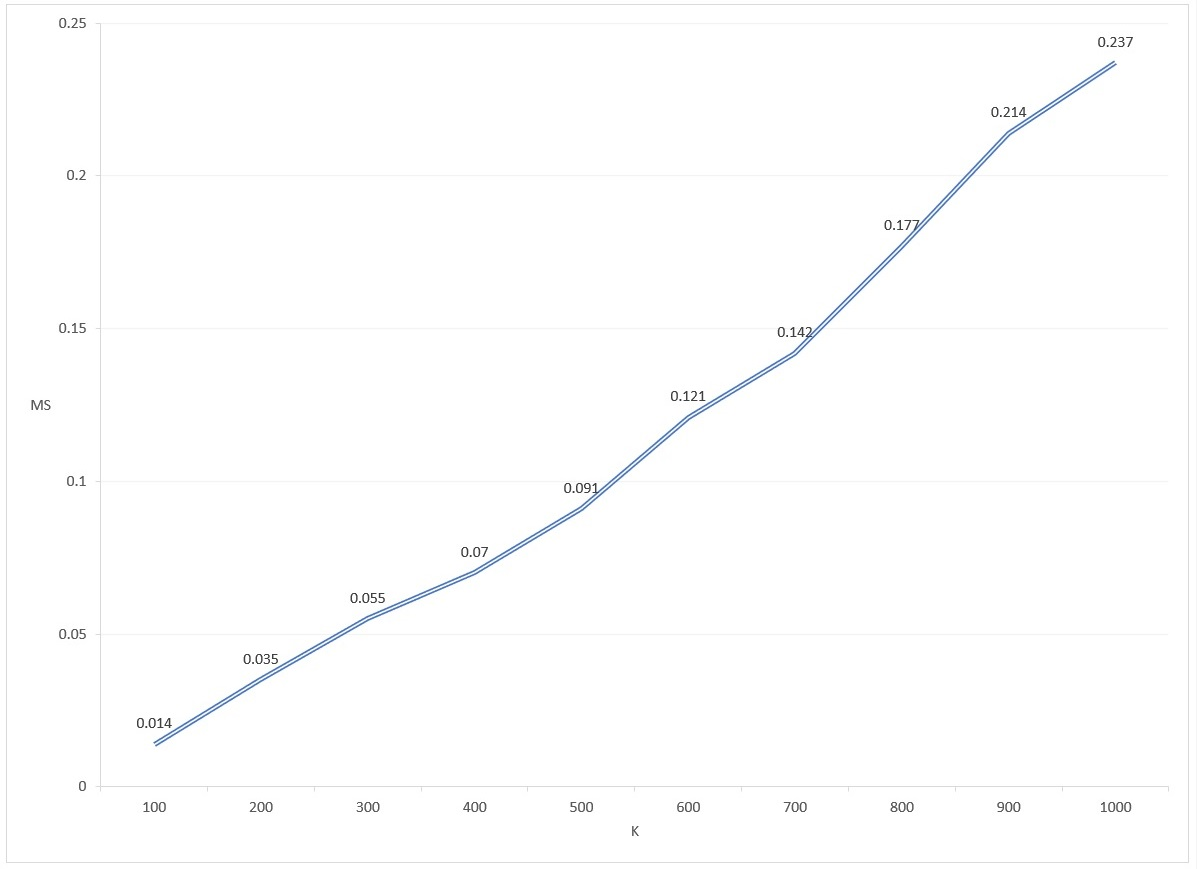
\includegraphics[scale=0.53]{graph.jpg}
    \end{minipage}
    
\caption{K-t 拟合曲线}
\end{figure}

\end{document}
